\chapter{RNA editingの検出手法の精度評価}
\section{研究背景}
RNA editingサイトの検出は、これまでにヒト、マウス、ショウジョウバエを主な対象生物種としてRNA-seqデータを用いた情報学的な手法が多数開発されている。RNA editingサイトはゲノムと転写物の一塩基のミスマッチとして検出されるが、シーケンシングやマッピングに起因した擬陽性を多く含む。そのため、真のRNA editingサイトと擬陽性とを高精度に分離させる検出手法がこれまでに考案されてきた。ところが、論文ごとに解析対象となる生物種や組織、セルライン、シーケンシング手法などに相違が見られ、各々の手法の検出精度の評価・比較は困難な状況にある。また多くの研究はこれまでに同定された既知のeditingサイトとの一致 (共通項)を確認しているに過ぎず、検出結果に含まれる擬陽性の影響を適切に評価するには至っていない。今後、RNA editingサイトを高精度に検出する手法を開発するにあたっては、既知の結果との一致と同時に、検出結果に含まれるノイズとその割合を評価する必要があると考えられる。バイオインフォマティクスの分野においては、タンパク質の立体構造予測コンテスト CASP (Critical Accesment of protein Structure Prediction)に代表されるように、その分野で開発されたアルゴリズムは、予測精度や計算時間といった複数の指標により性能評価が行われ、手法の標準化が行われてきた経緯を持つ。本研究もこういった文脈に位置づけることができる。
\par
異なる検出手法について、何らかの指標による精度評価は、生物種やサンプルごとにおいて高精度な検出に寄与するパラメータとその値が明らかとなる。序論で前述したとおり、RNA editingサイトの高精度な検出には、様々なフィルタリング手法を複合的に組み合わせることによって擬陽性の排除が行われており、検出手法ごとにゲノムへのマッピング時における許容ミスマッチ数から、擬陽性の減少に有効的なフィルタリング方法が異なる。高精度な検出手法が明らかとなると、他の手法との差を高精度な検出に寄与するパラメータの候補として抽出することが可能である。このような知見は、汎用性のある新たなRNA editingサイトの検出手法の開発に貢献することを期待する。本研究は、ヒト・マウス・ショウジョウバエのRNA-seqデータを用いた既存の検出手法対して、性能評価を行い高精度な検出に寄与するパラメータの探索を行ったものである。性能評価には再現率・適合率といった指標を導入し、各手法の検出精度について定量的な比較を行った。結果、検出手法それぞれの持つ検出精度を明らかにし、シーケンシング手法などの実験デザインおよび検出手法が検出精度にどのように寄与しているのかについて議論する。
\newpage
\section{対象と手法}
\subsection{性能評価に用いた指標}
これまでに開発されてきたRNA editingサイトの検出手法を統一的な指標によって性能評価を行うため、適合率 (Precision)・再現率 (Recall)・F値 (F-measure)と呼ばれる3つの指標を導入した。この3つの指標は情報工学において検索精度の測定において用いられており、情報検索の結果に対して検索ノイズと検索漏れという2つの側面から検出器の性能を測定するものである。以下にぞれぞれの指標とその計算方法について示す。この3つの指標は、算出される値が高いほど高精度であることを表す。以下で説明する際の検出サイトは、各手法により検出された全A-to-I editingサイトを指し、正解サイトは過去に報告された既知の全editngサイトを表す。
\par
適合率は、式\ref{eq:precision}に定義される。検出サイトと真のeditingサイトの積集合に対する検出サイトの割合として計算される。適合率は検出サイトに正解が含まれる割合を意味しており、検出サイトの中に正解サイトとの一致が濃縮されることで高い適合率が達成される。
\begin{eqnarray}
	Precision = \frac{TP}{TP + FP} = \frac{CandidateSites \cap TrueEditingSites}{CandidateSites}
	\label{eq:precision}
\end{eqnarray}
\par
再現率は、式\ref{eq:recall}に定義され、正解セットに対して検出サイトが正解した割合を示す。ゲノム中における多くの箇所をedititingサイトとして検出することで原理的に再現率は1に近づくが、一方で擬陽性が増大するため適合率は0に近づく。このように、両者はトレードオフの関係にあることから、正確なRNA editingサイトの検出には、再現率の向上よりも高い適合率を示す手法やパラメータを見出すことが重要となる。
\begin{eqnarray}
	Recall = \frac{TP}{TP+FN}
	= \frac{CandidateSites \cap TrueEditingSites}{TrueEditingSites}
	\label{eq:recall}
\end{eqnarray}
\par
F値は、適合率および再現率の調和平均として式\ref{eq:f_measure}のように定義される。F値の導入により、再現率と適合率の2つの評価基準を一元的に取り扱うことが可能となる。
\begin{eqnarray}
	Fmeasure = 2 \times \frac{precision \times recall}{precision + recall}
	\label{eq:f_measure}
\end{eqnarray}
\subsection{正解セットの構築}
検出精度を評価するためには、真のRNA editingの集合を定義した正解セットの構築が必須となる。そこで、これまでの研究によって報告されたA-to-I editingサイトを収集したDARNED (DAtabase of RNa EDiting site, \url{http://darned.ucc.ie/})と呼ばれるデータベースに登録されている全データをヒト・マウス・ショウジョウバエの3種ごとに取得し、正解セットとした。DARNEDは、実験的な手法により同定されたA-to-I editingサイトの他に、情報学的な手法により同定されたサイトの双方を含み、文献と紐付けられたeditingサイトに関するメタデータと共に公開している。表\ref{tab:darned}に、生物種ごとに収集した正解セットの総数をまとめた。尚、精度評価の実施にあたり、取得した全てのサイトを正解セットとして扱い、同定手法の如何については区別しなかった。
\begin{longtable}{cccc}
	\vspace{-0.5cm}
	\label{tab:darned}\\
	\caption{DARNEDより収集したA-to-I editingサイトの内訳}\\
	\cline{1-4}
	\bf{Species} & \bf{Reference genome version} & \bf{Studies} & \bf{Answer sites} \\
	\cline{1-4}
	\it{H. sapiens} & hg19 & 20  & 333,216 \\
	\it{H. sapiens} & hg18 & 22  & 259,705 \\
	\it{M. musclus} & mm10 & 4   & 8,341 \\
	\it{M. musclus} & mm9  & 4   & 8,352 \\
	\it{D. melanogaster}   & dm3 & 3 & 1,969 \\
	\cline{1-4}
	\vspace{-0.8cm}
\end{longtable}
\begin{flushleft}
	\small{DARNEDにより取得した3種それぞれの正解セットを示す。3種それぞれに対応するゲノムのバージョン、editingサイトが同定された先行研究の数、収集した正解セットの総数をそれぞれ示す。}
\end{flushleft}

\subsection{精度検証に用いられた既存の検出手法}
RNA editingサイトの検出精度に関する性能評価を実施するにあたり、(i) RNA-seqデータを用いた検出手法であること、(ii) シーケンスデータがSequence Read Archive (\url{http://www.ncbi.nlm.nih.gov/sra/})において公開されていること、(iii) 同定されたRNA editingサイトの全リストが取得可能であることを評価の条件とし、ヒト・マウス・ショウジョウバエの3種類からそれぞれ評価する先行研究を選出した。表\ref{tab:methods}にその一覧を示した。一覧では、便宜的に先行研究ごとに分類しているが、先行研究によっては異なる組織やセルラインに多数の解析を行っている場合があるため、この場合に関してはサンプルごとに性能比較を行うようにした。これにより同一手法における組織やセルライン毎での精度の違いを明らかにすることができると考えられた。
\begin{longtable}{cccc}
	\vspace{-0.5cm}
	\label{tab:methods}\\
	\caption{性能評価に用いた検出手法のリスト}\\
	\cline{1-3}
	\bf{Study} & \bf{Samples (tissue/cell line)} & \bf{Identified sites} \\
	\bi{H. sapiens} \\
	\cline{1-3}
	%\endhead
	Ramaswami, \it{et al.,} \rm{2012} & GM12878 (lymphoblastoid cell line)                    & 74,166 \\
	Ramaswami, \it{et al.,} \rm{2013} & lymphocyte cell line                                  & 230,402 \\
	Peng, \it{et al.,}             \rm{2012} & lymphoblastoid cell line in Han Chinese individual    & 22,696 \\
	Park, \it{et al.,}             \rm{2013} & 14 human cell lines (ENCODE project)                  & 13,821 \\
	Zhu, \it{et al.,}              \rm{2013} & 16 human tissues, 2 cell lines (Illumina BodyMap 2.0) & 2,246 \\
	Bahn, \it{et al.,}            \rm{2012} & U87MG (glioblastoma cell line)                        & 12,791 \\
	\bi{M. musculs} \\
	\cline{1-3}
	Gu, \it{et al.,} \rm{2012}         & White adipose, Femurs, liver      & 244 \\
	Dillman, \it{et al.,} \rm{2013}    & Cerebral cortex, 4 embryonic mice & 177 \\
	Lagarrigue, \it{et al.,} \rm{2013} & Liver, Adipose                    & 363 \\
	\bi{D. melanogaster} \\
	\cline{1-3}
	Rodriguez, \it{et al.,} \rm{2012} & Fly head & 1,351 \\
	Graveley, \it{et al.,} \rm{2011}  & Fly head & 973 \\
	Ramaswami, \it{et al.,} \rm{2013} & Fly head & 850 \\
	\cline{1-3}
	\vspace{-0.8cm}
\end{longtable}
\begin{flushleft}
	\small{本研究において精度評価の対象となった先行研究の検出手法を生物種ごとに分類して示した。先行研究が用いたセルラインや組織と最終的なA-to-I editing候補サイトの総数を表記した。異なるセルラインや組織の結果を統合的に解析している場合は、複数を列挙した。}
\end{flushleft}
\section{検出性能の比較結果}
\subsection{ヒトを対象とした検出手法}
ヒトを対象とした性能評価の結果、対象とした検出手法の全体としての精度の傾向は、どの手法も再現率が0.2以下と低く、適合率は手法とサンプルによって大きく分散することが示された (図 \ref{fig:human_cr})。最も高い再現率を示した手法は、Ramaswami et al., 2012であり、適合率に関してはPeng et al., 2012であった。対して、最小の再現率と適合率を示した手法は、脳における反復配列領域以外の領域を検出したRamaswami et al., 2013の手法であった。ENCODEプロジェクトにおいて用いられた手法は、どのセルラインに対しても低い精度を示す傾向が見られた。
\par
手法ごとに再現率、特に適合率が大きく分散する傾向が観察された要因について探るため、再現率・適合率と候補サイトの総数との関連性についての解析を行った (図\ref{fig:human_data})。その結果、再現率および適合率の双方は、検出サイト数の増大に対応して、精度も向上する傾向が示された。
\begin{figure}[htbp]
	\begin{center}
		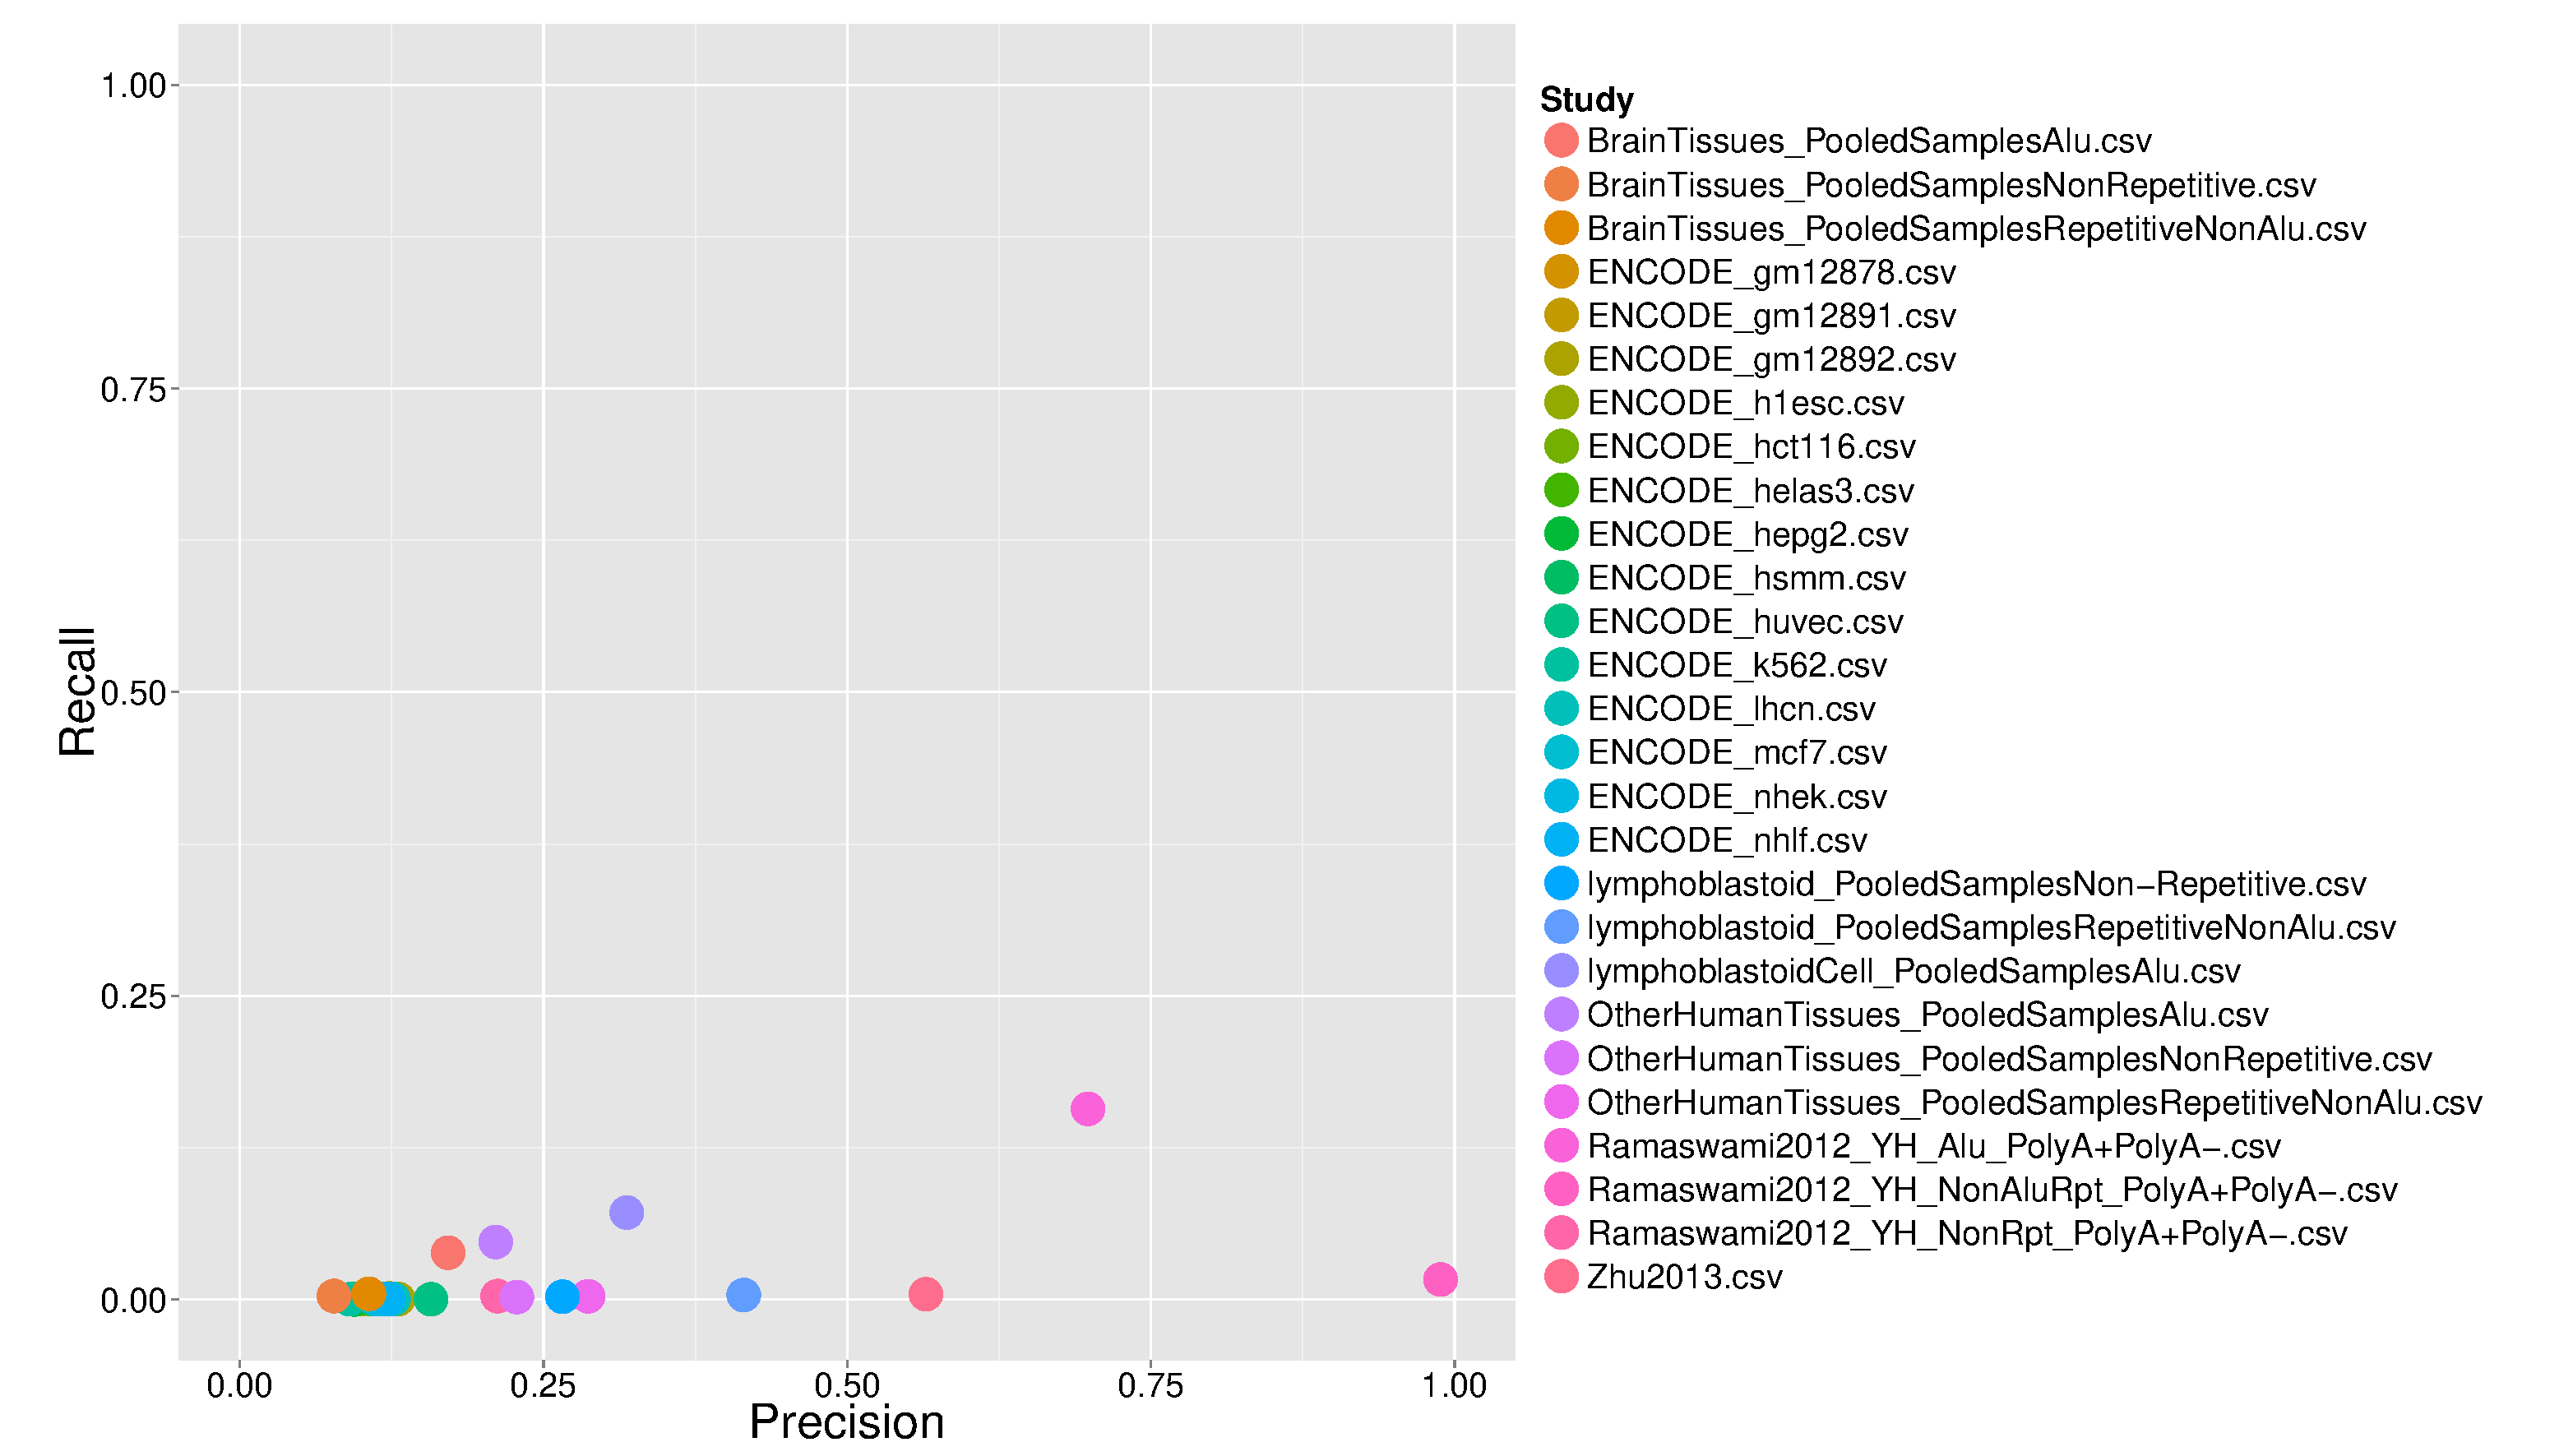
\includegraphics[width=0.70 \hsize]{bench_human.pdf}
	\end{center}
	\caption{ヒトにおける検出精度の評価結果}
	\vspace*{-0.2cm}
	\begin{flushleft}
		\small{ヒトを対象とした手法の性能評価の結果を示す。横軸に適合率、縦軸に再現率をそれぞれ示した。図中の色分けは、手法あるいはセルラインや組織ごとに変えて表した。}
	\end{flushleft}
	\label{fig:human_cr}
\end{figure}
\begin{figure}[htbp]
	\begin{center}
		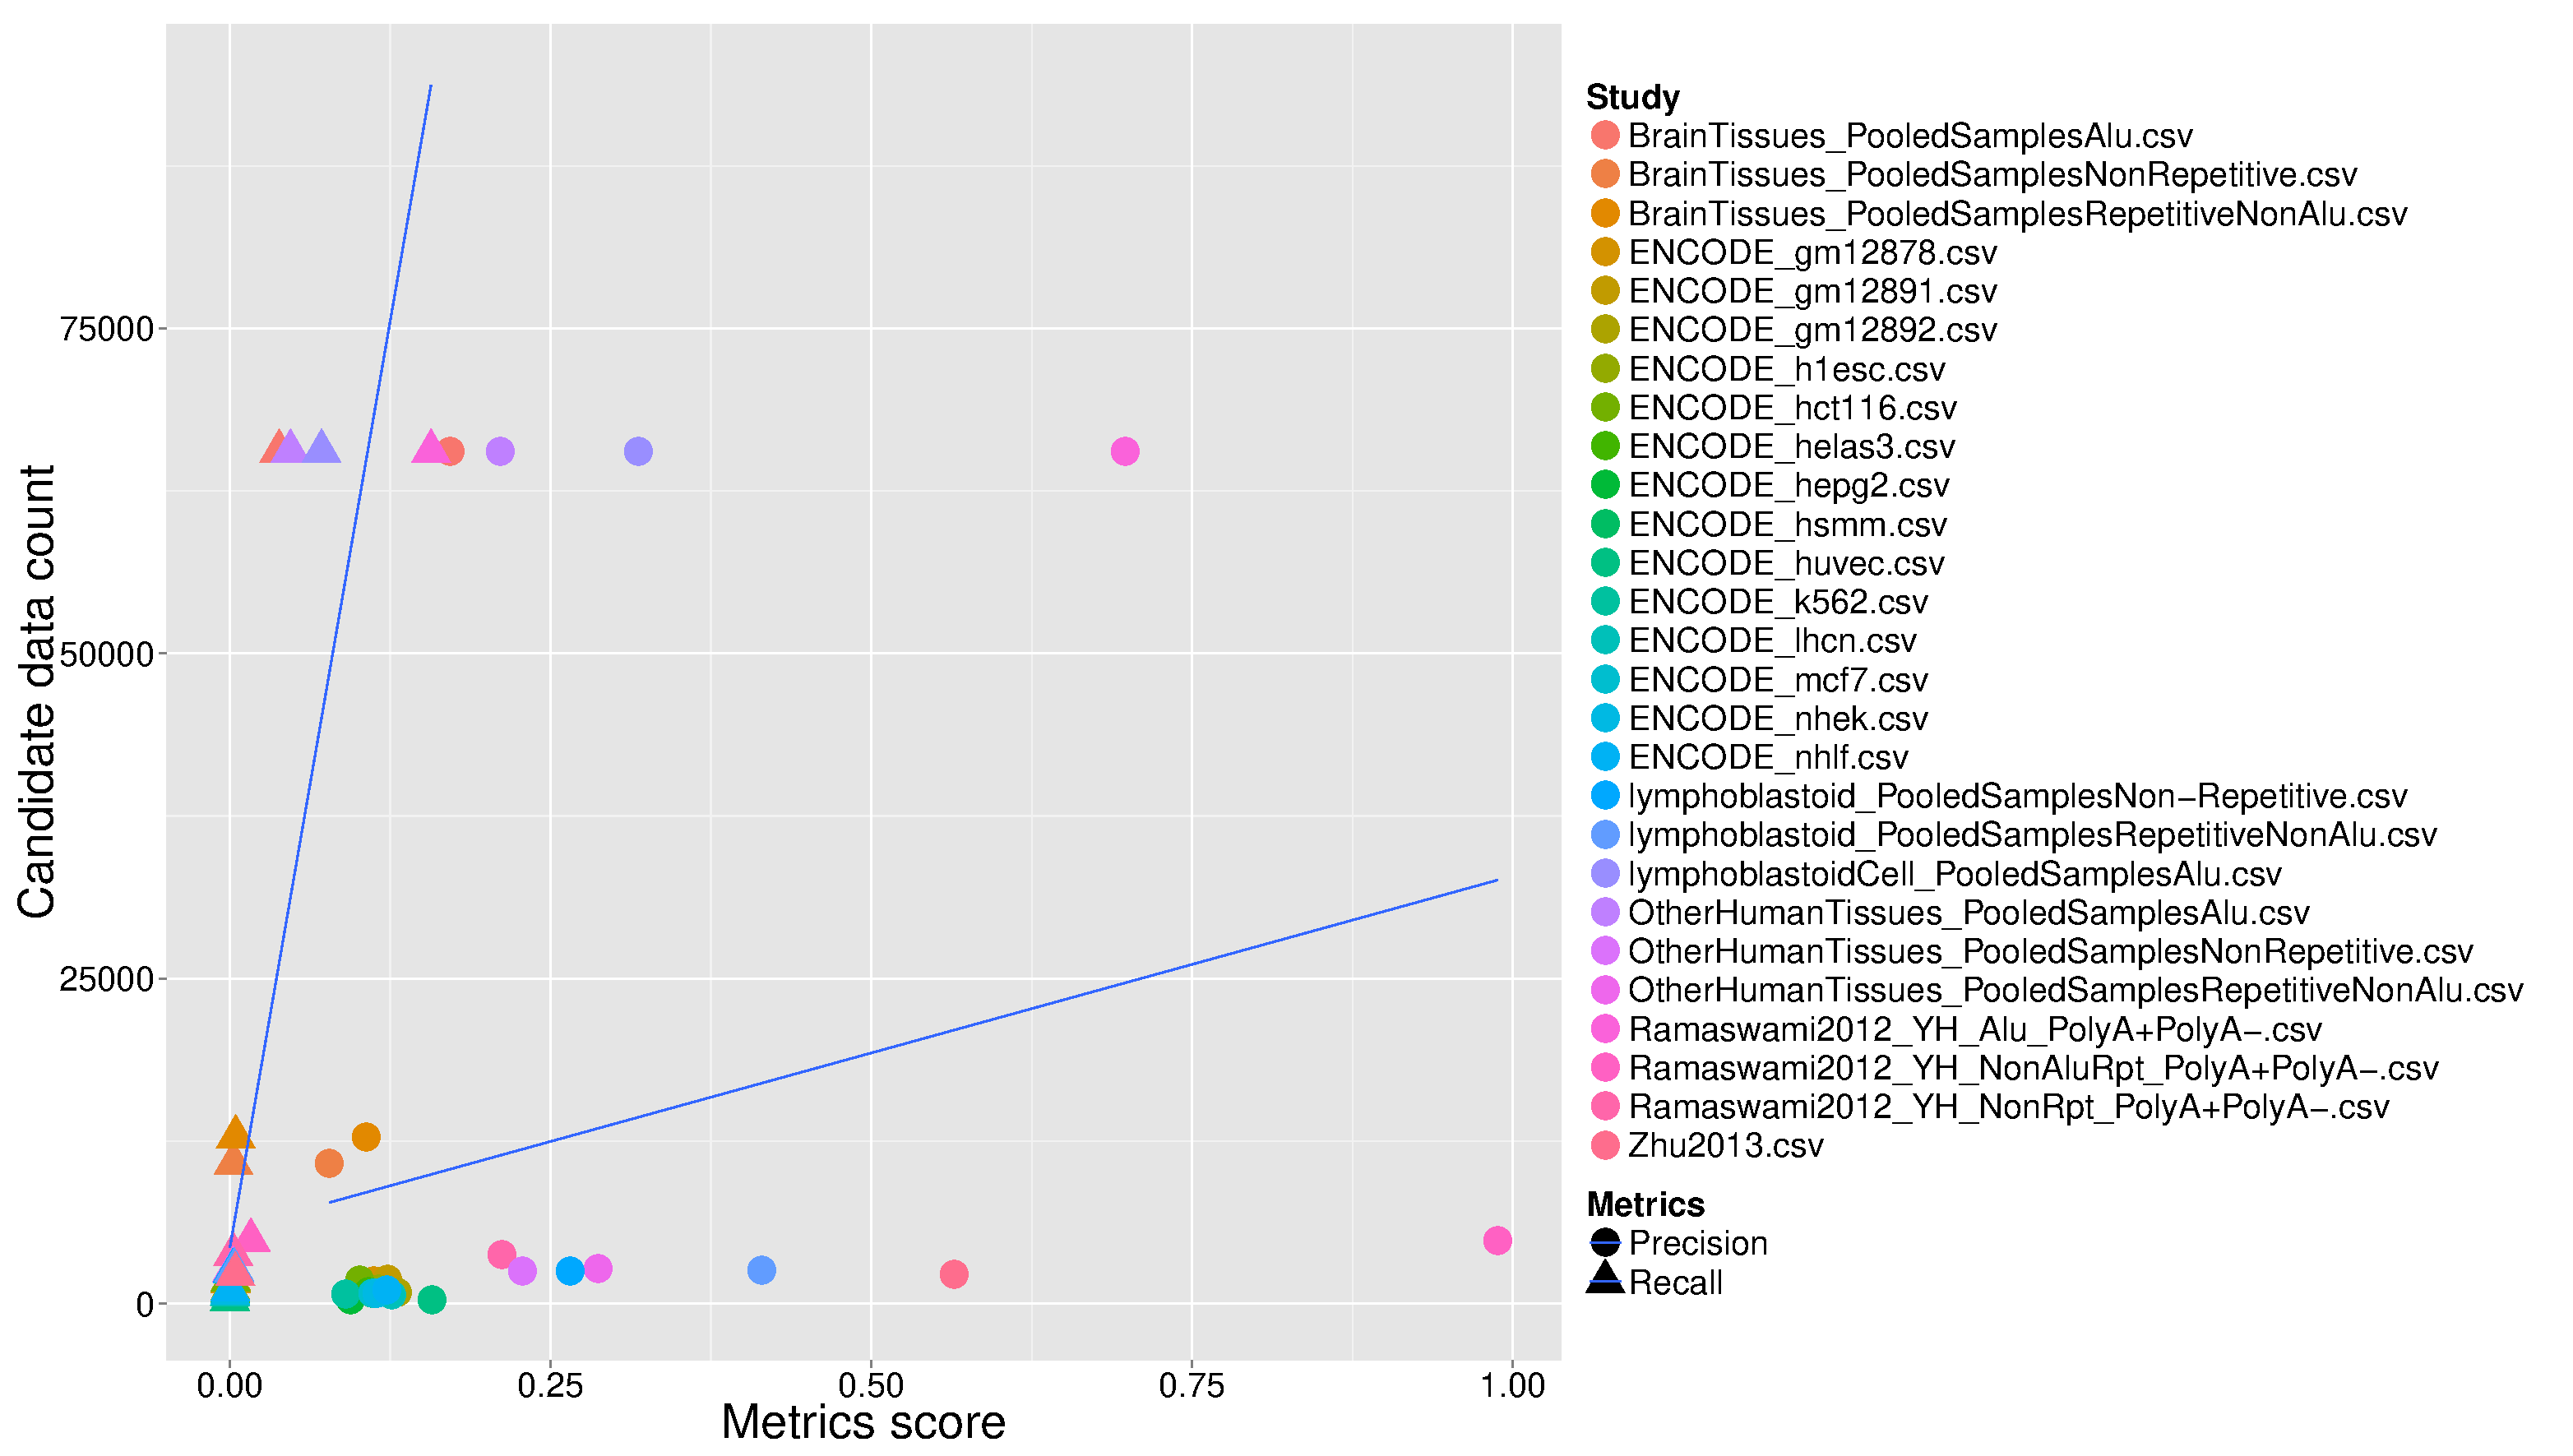
\includegraphics[width=0.70 \hsize]{Human_correlation.pdf}
	\end{center}
	\caption{ヒトにおける検出精度と候補editing数との関係性}
	\vspace*{-0.2cm}
	\begin{flushleft}
		\small{ヒトを対象とした手法について、縦軸にそれぞれの手法によって検出されたA-to-I editingサイト数を示し、横軸に適合率および再現率を図示した。検出精度の指標はそれぞれ黒丸は適合率、黒三角は再現率に対応する。また、青線は適合率および再現率と候補サイト数の回帰直線を示す。}
	\end{flushleft}
	\label{fig:human_data}
\end{figure}
\newpage
\subsection{マウスを対象とした検出手法}
マウスを対象とした検出手法の性能評価の結果を図\ref{fig:mouse_data}に示した。紫丸で示したGu et al (2012)が最大の再現率、0.99を示した。また、3つの手法全てに共通して再現率が低いことが示された。Gu et al (2012)は、マウスの肝臓から抽出されたサンプルを用いたRNA-seqデータからA-to-I editingサイトを検出している。手法ごとの候補サイトの検出数と精度の関係については、図\ref{fig:mouse_data}に示した。2つの手法に関しては、ヒトやショウジョウバエと同様に検出数に応じて精度が向上する傾向が見られた。
\begin{figure}[htbp]
	\begin{tabular}{cc}
		\begin{minipage}{0.5\hsize}
				\centering
				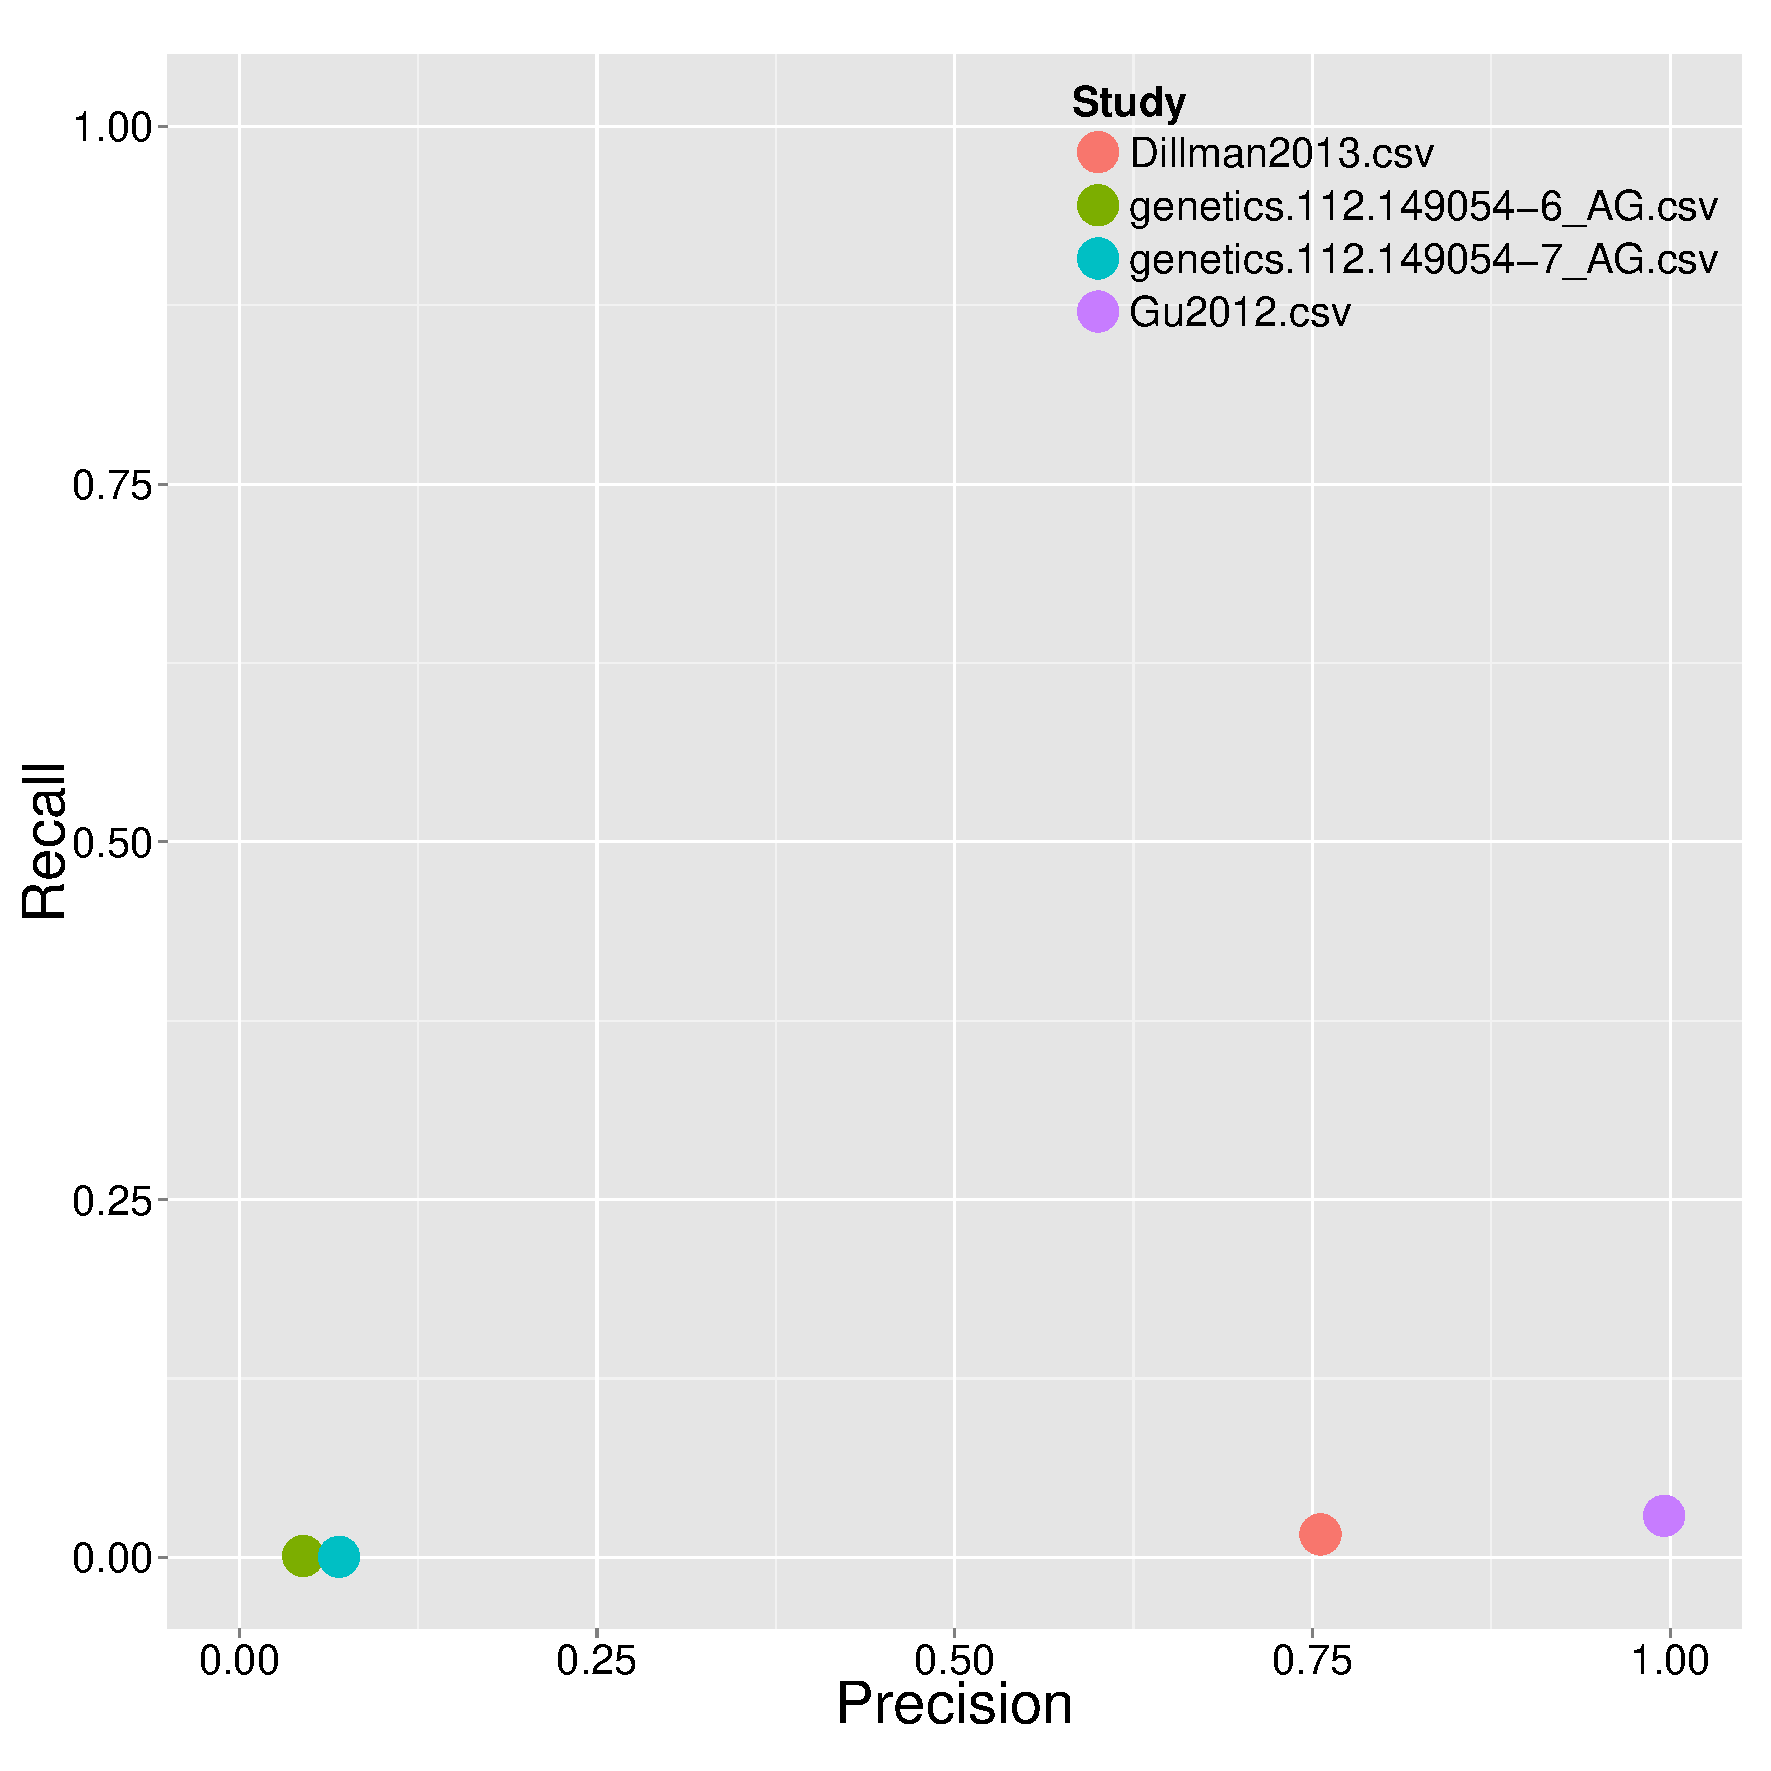
\includegraphics[width=1.0 \hsize]{bench_mouse.pdf}
				\label{fig:dmel_pr}
		\end{minipage}
		\begin{minipage}{0.5\hsize}
				\centering
				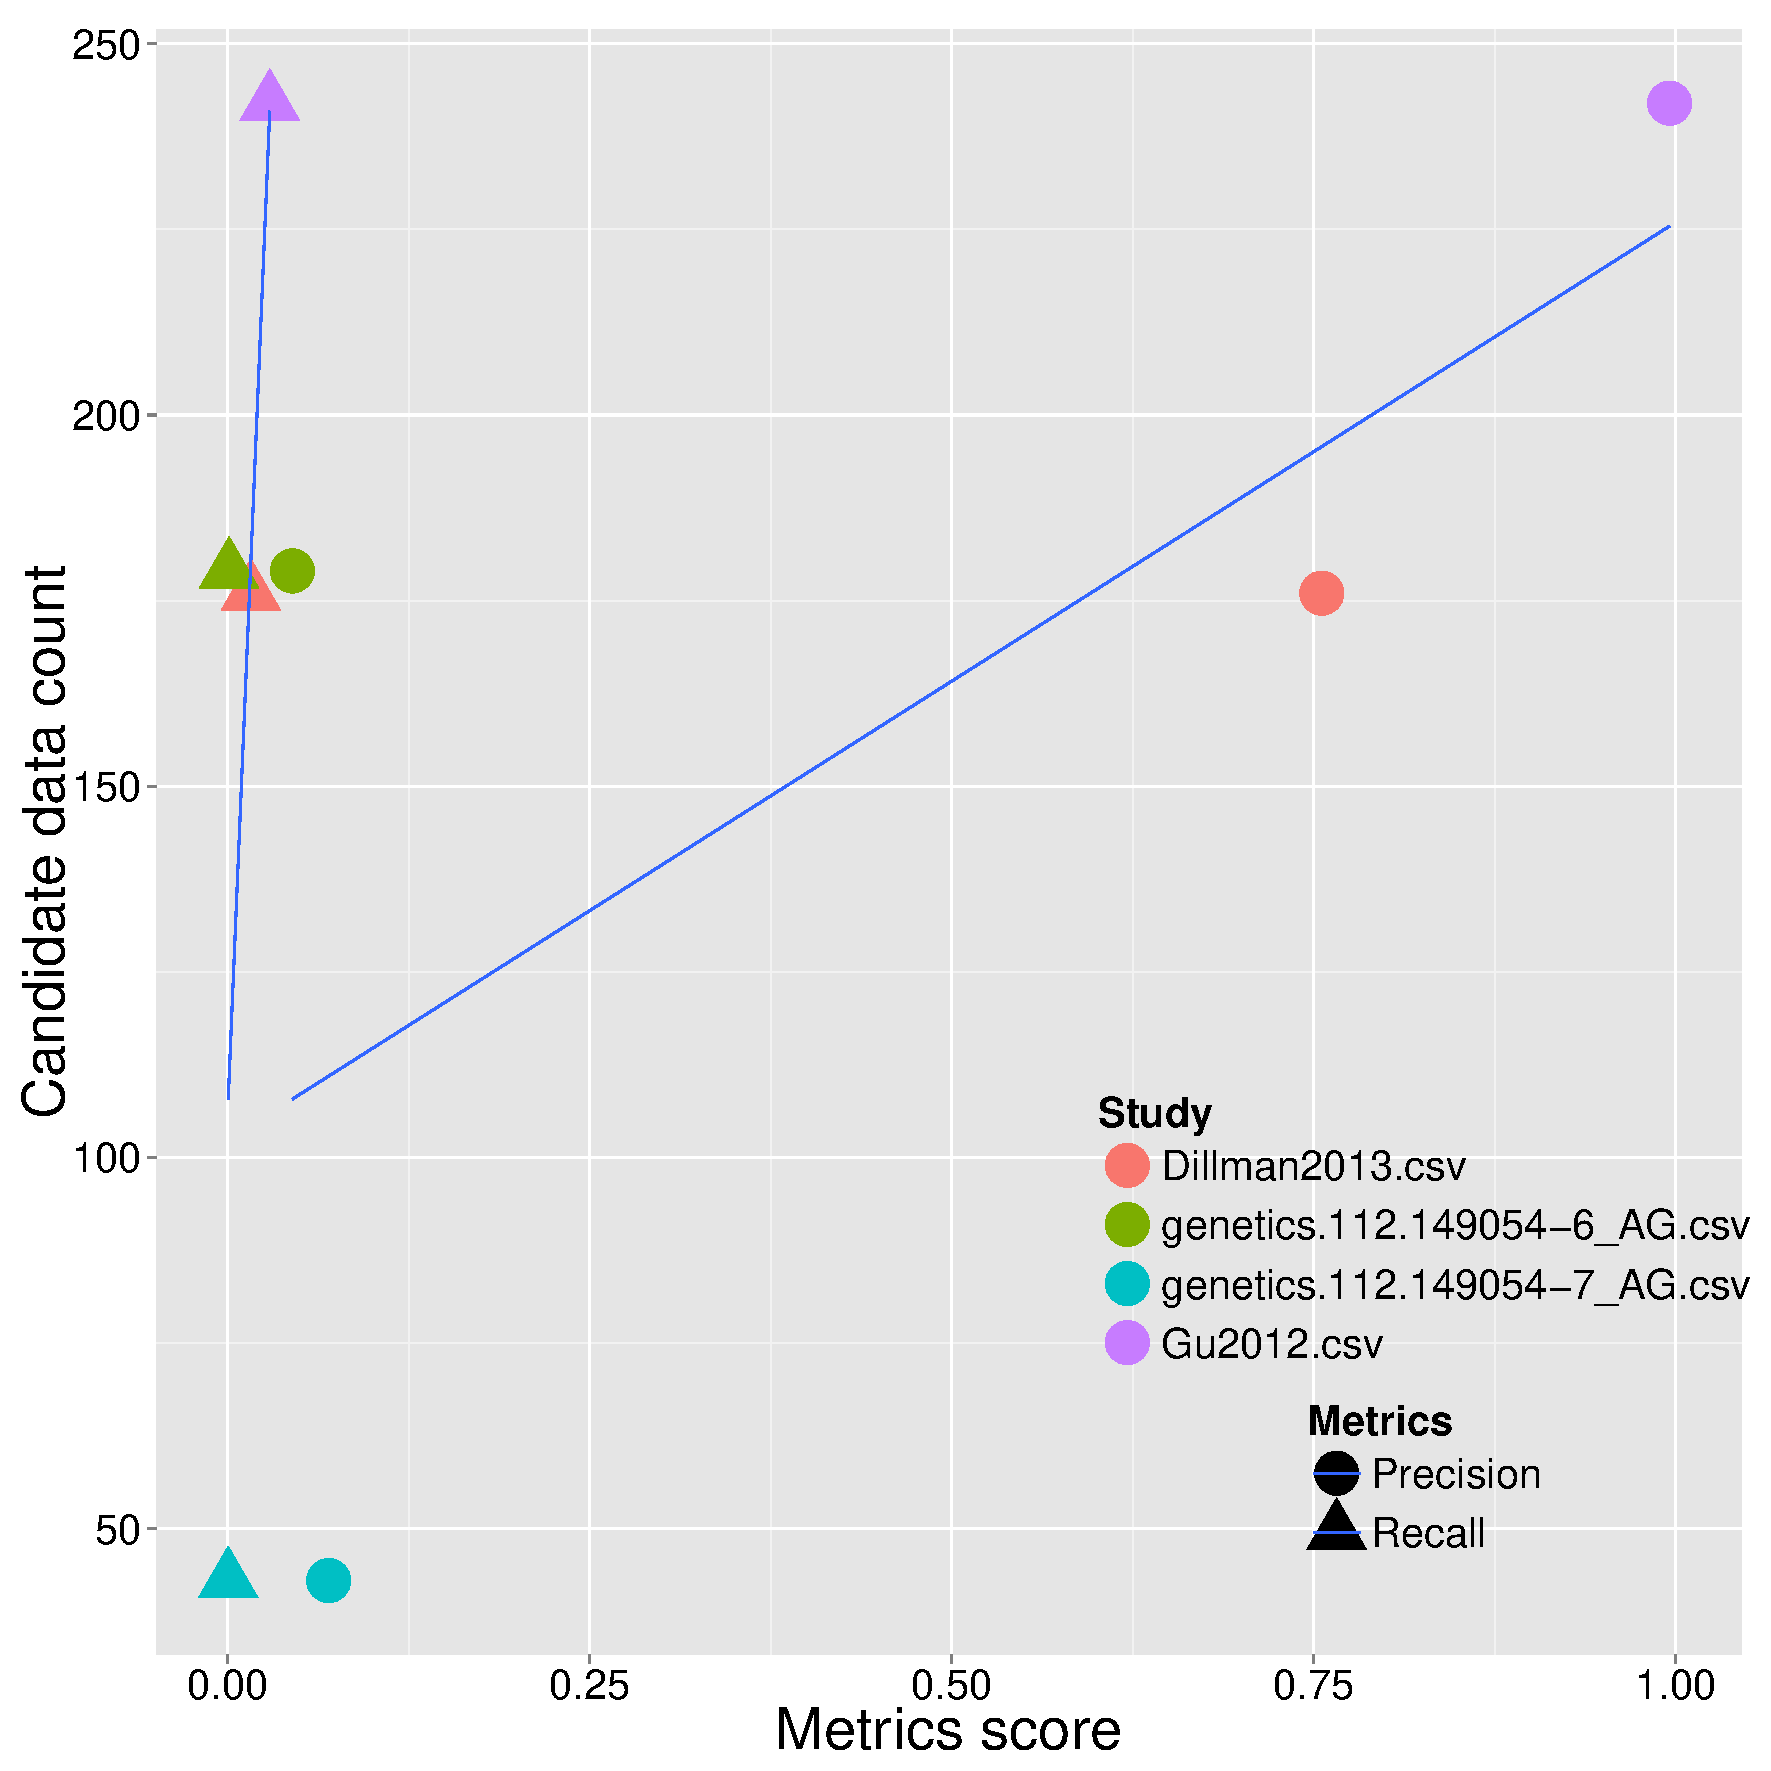
\includegraphics[width=1.0 \hsize]{Mouse_correlation.pdf}
				\label{fig:dmel_cor}
		\end{minipage}
	\end{tabular}
	\caption{マウスのデータを用いた検出手法の精度評価}
	\vspace*{-0.2cm}
	\begin{flushleft}
		\small{A: マウスにおける検出精度の結果を示す。B: 候補となったA-to-I editingサイト数と検出精度との関係性を示す。青線は、候補サイト数と検出精度の回帰直線を示す。}
	\end{flushleft}
	\label{fig:mouse_data}
\end{figure}
\subsection{ショウジョウバエを対象とした検出手法}
ショウジョウバエを対象とした検出手法の精度比較の結果を図\ref{fig:dmel_data}に示す。最大の適合率を示した手法はRodriguez et al., 2012、再現率に関しては、modENCODEの手法が最大を示した。また、Ramaswami \it{et al}\rm{}., 2013において用いられた検出手法は、再現率ならびに適合率はどちらも他2つの手法に対して低い精度であることが示された。また、図\ref{fig:dmel_data}に示したように、候補となるeditingサイトを多く検出した手法ほど、再現率と適合率が向上するという傾向が確認された。
\begin{figure}[htbp]
	\begin{tabular}{cc}
		\begin{minipage}{0.5\hsize}
				\centering
				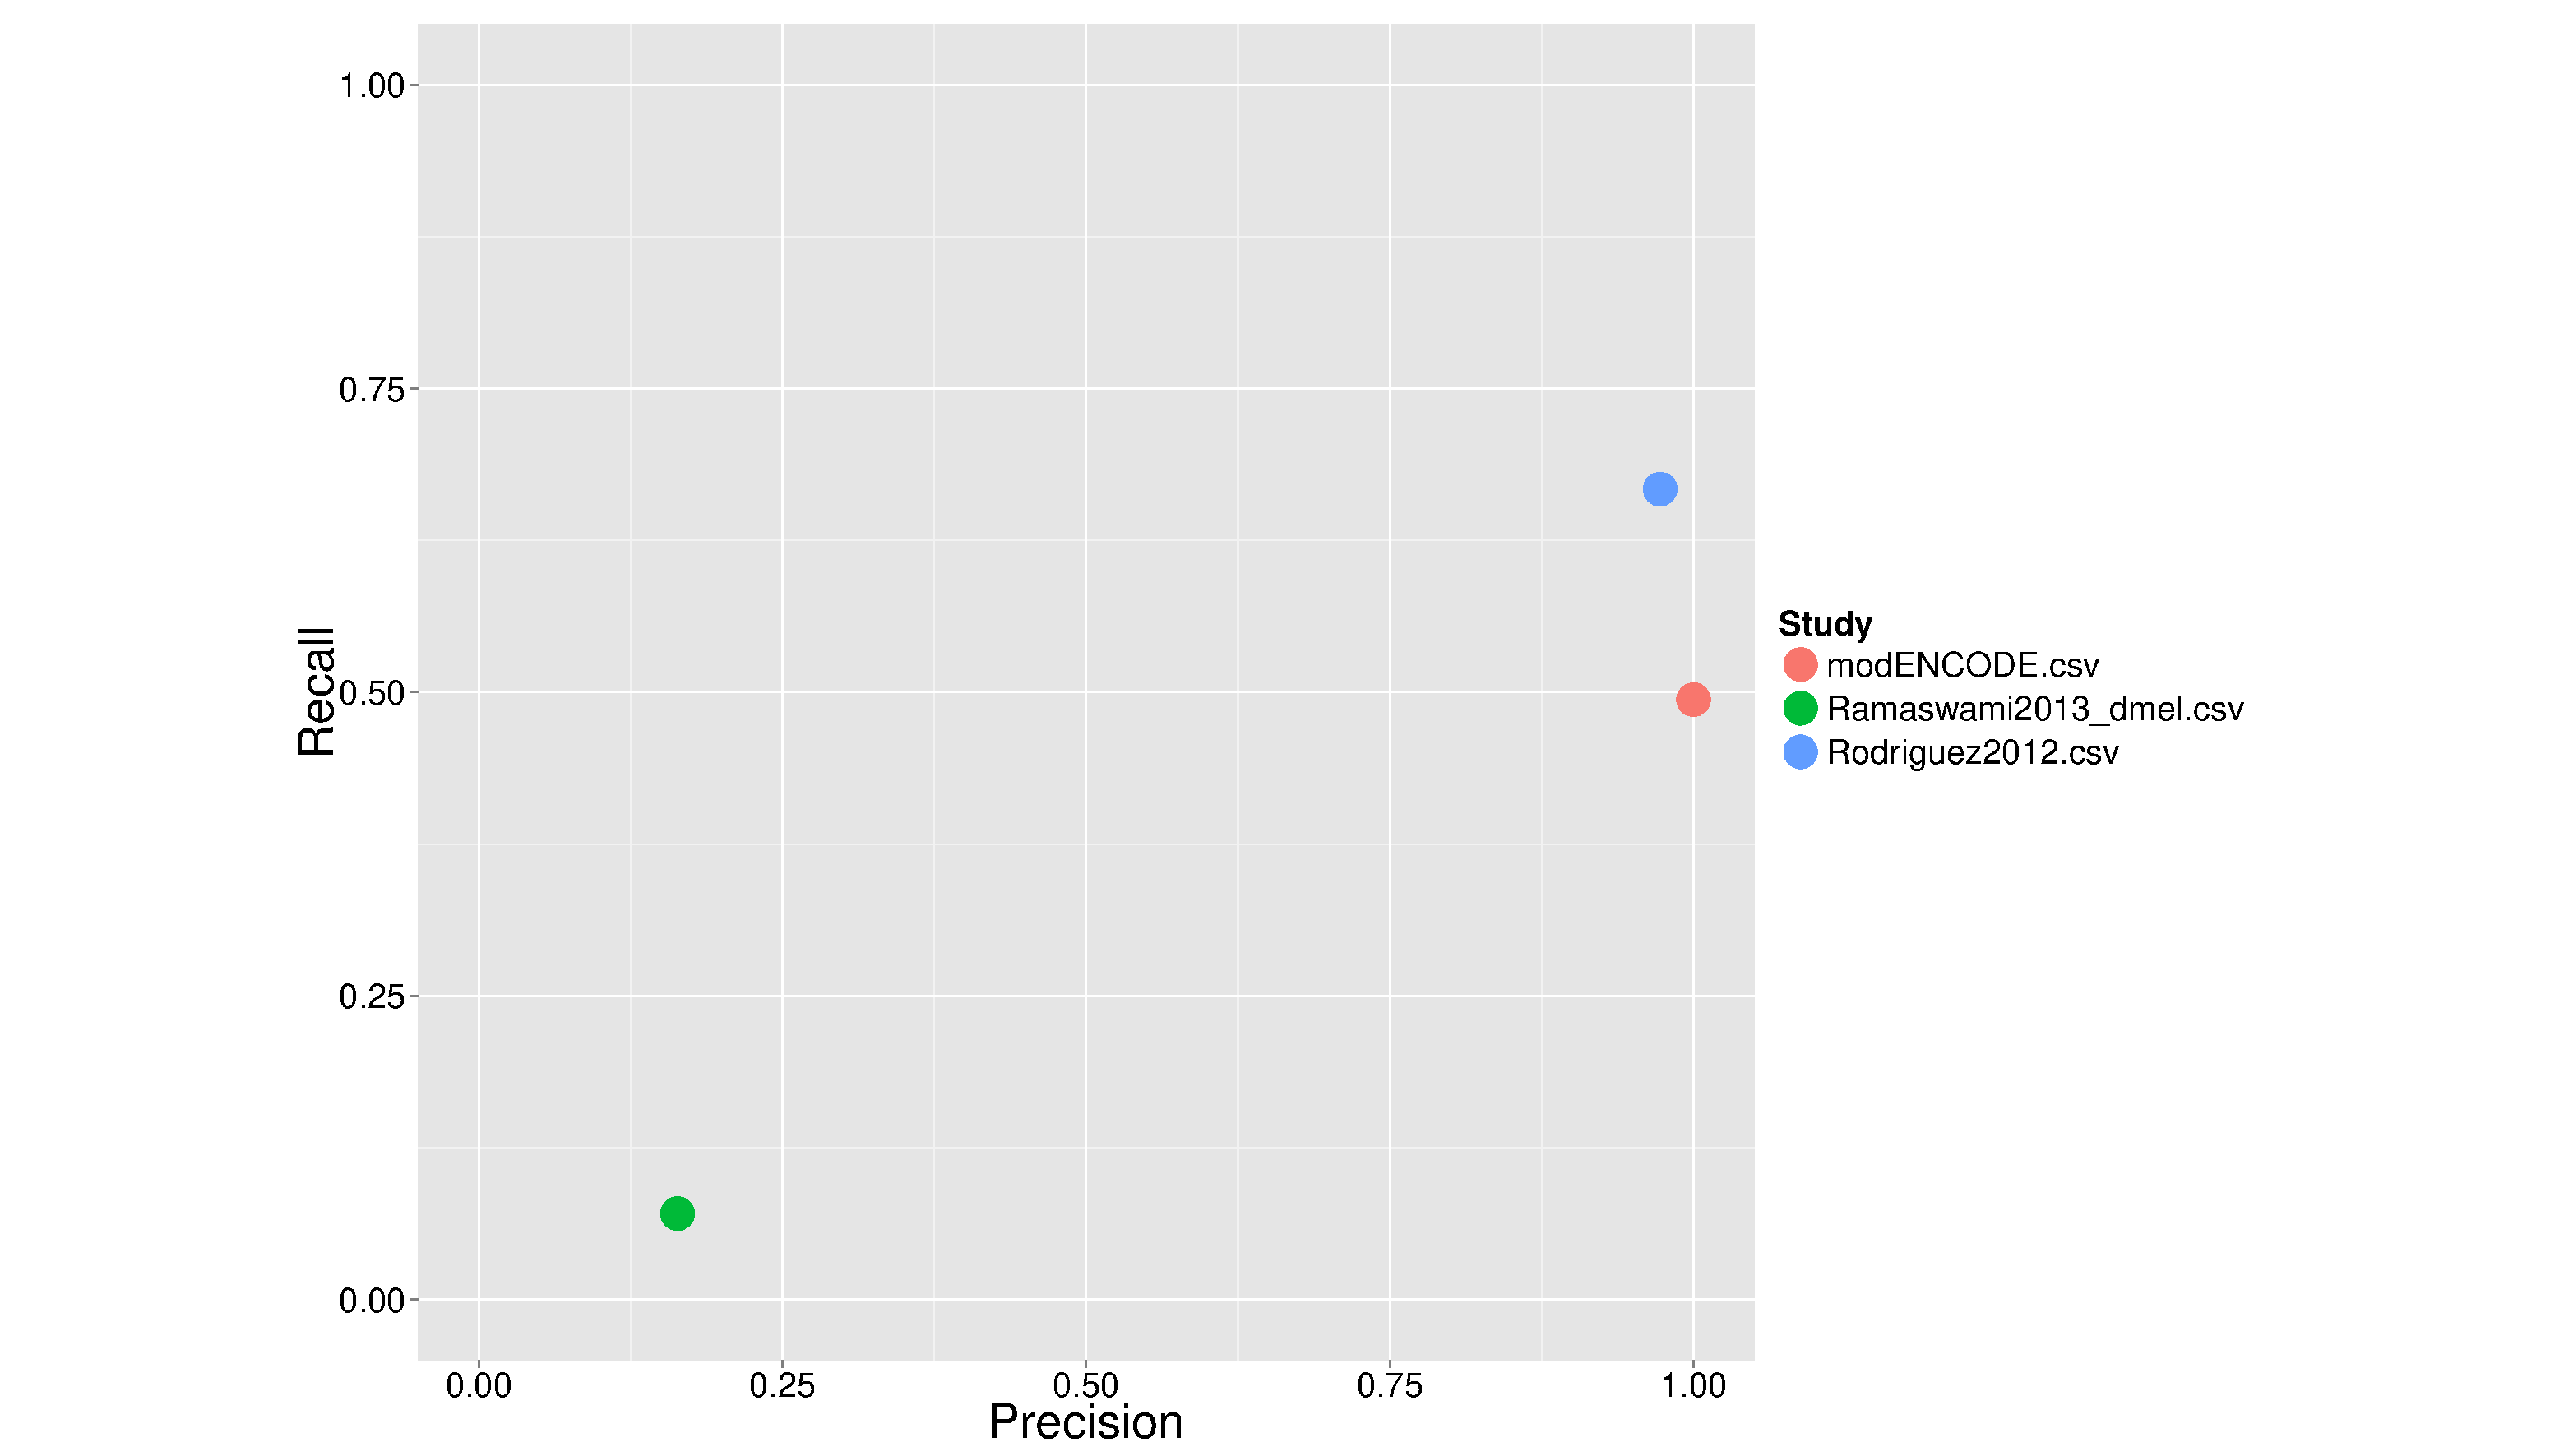
\includegraphics[width=1.0 \hsize]{bench_fly.pdf}
				\label{fig:dmel_pr}
		\end{minipage}
		\begin{minipage}{0.5\hsize}
				\centering
				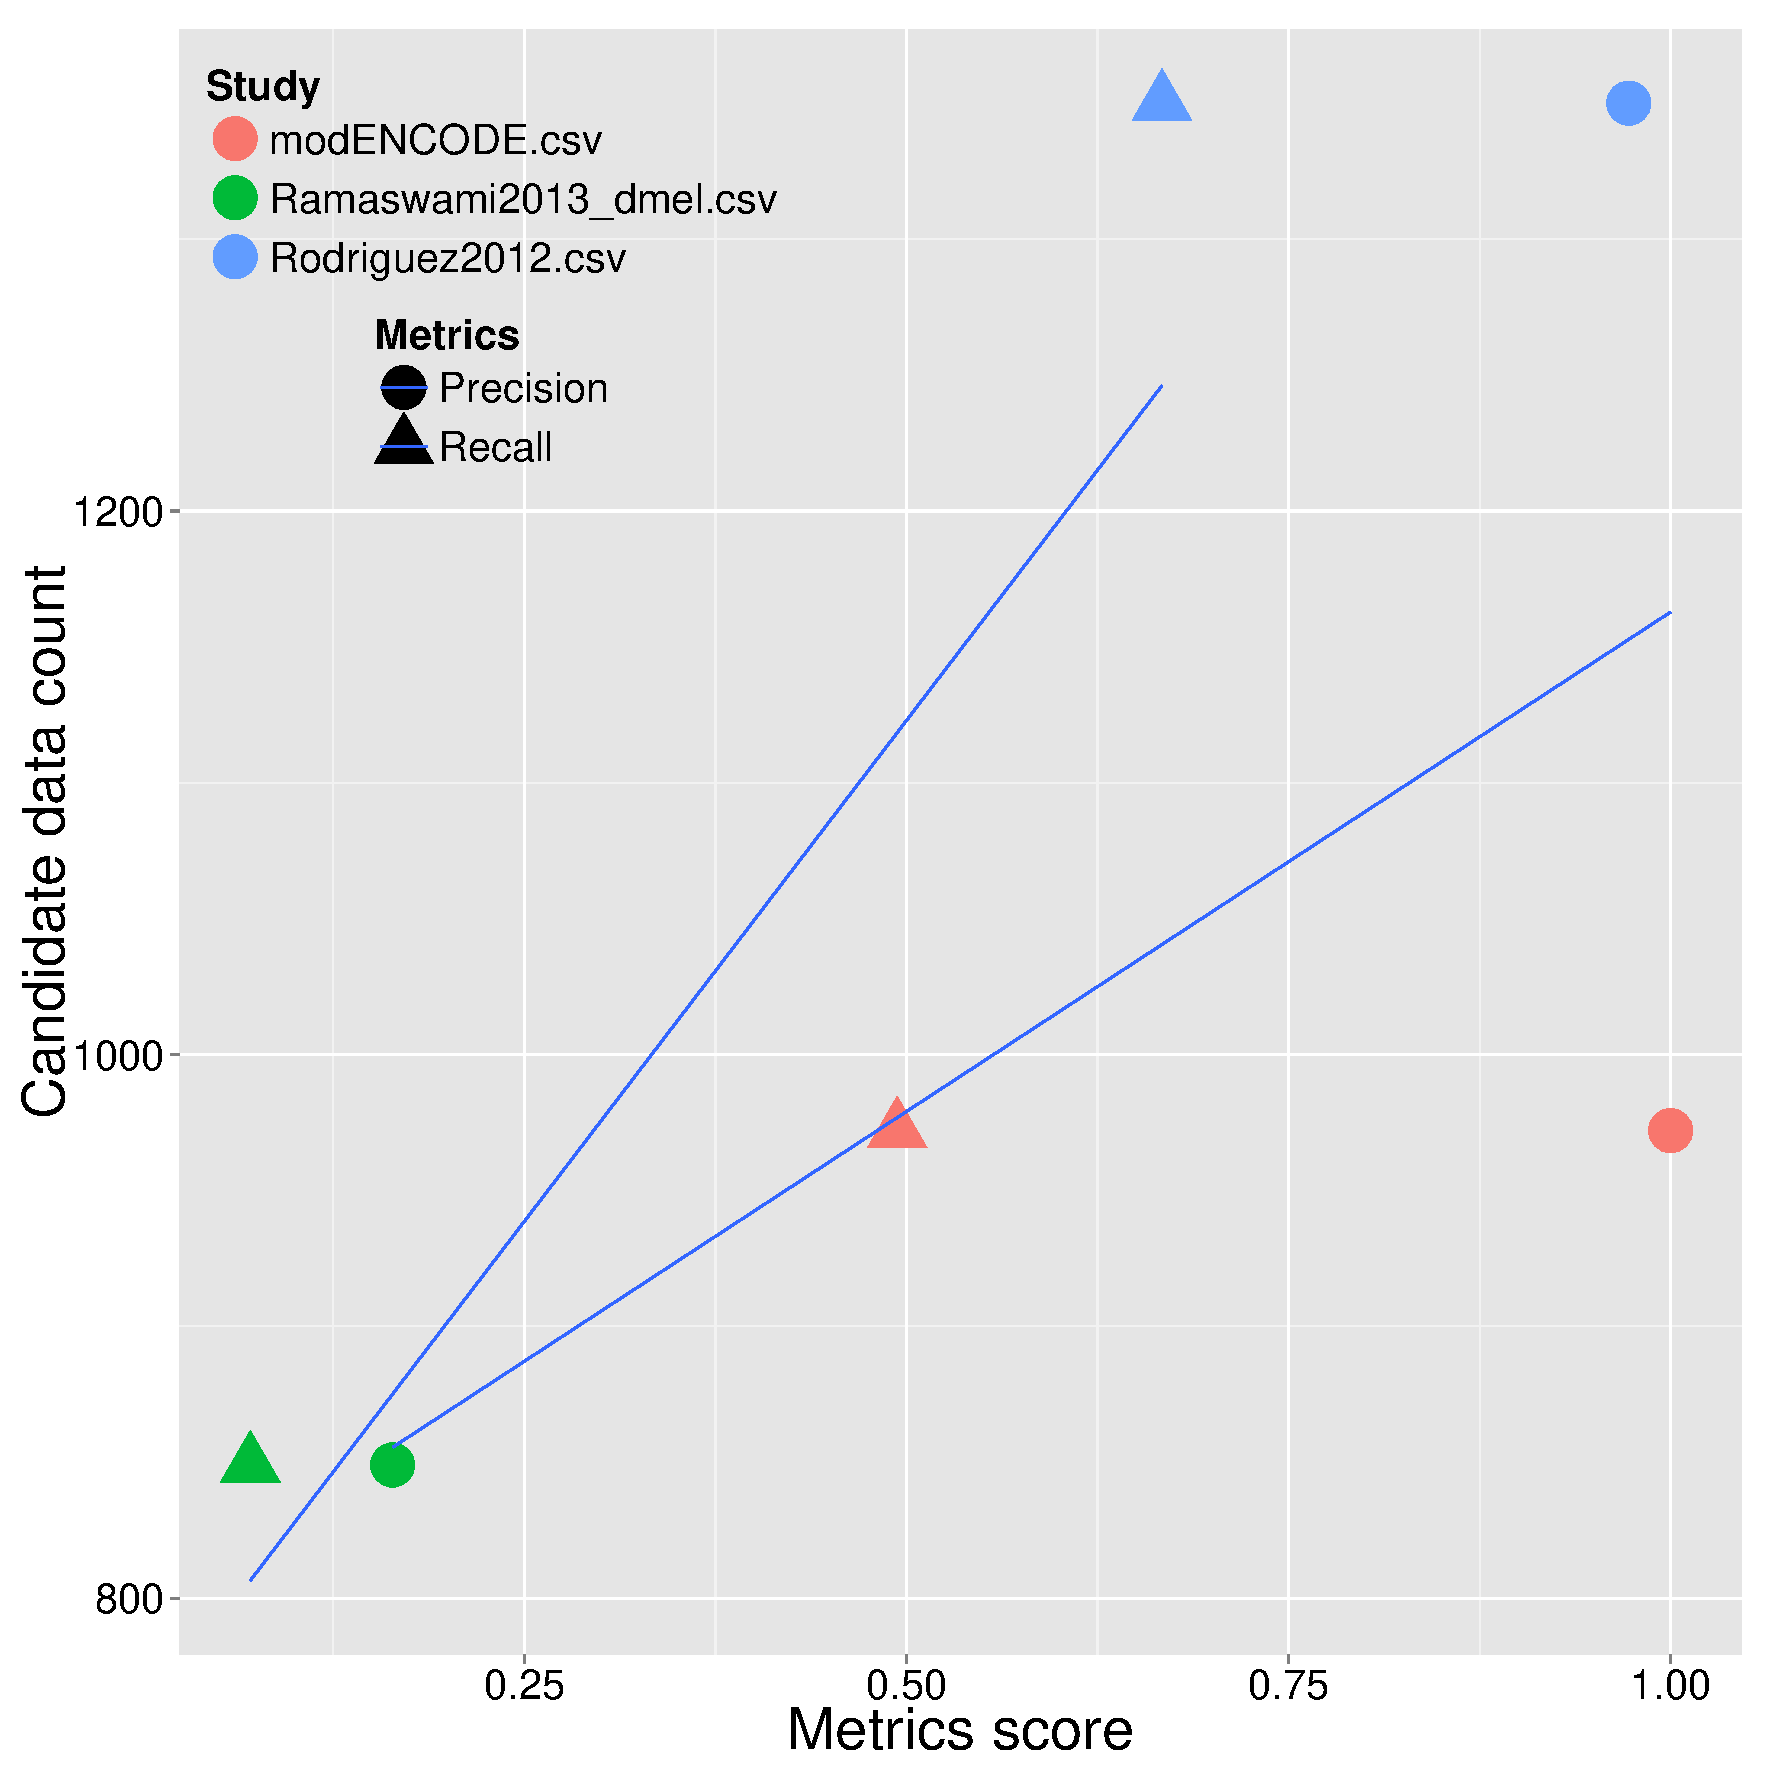
\includegraphics[width=1.0 \hsize]{dmel_correlation.pdf}
				\label{fig:dmel_cor}
		\end{minipage}
	\end{tabular}
	\caption{ショウジョウバエにおける検出手法の精度評価}
	\vspace*{-0.2cm}
	\label{fig:dmel_data}
	\begin{flushleft}
		\small{A: ショウジョウバエにおける各検出手法の精度結果を示す。B: 検出サイト数と適合率 (黒丸)および再現率 (黒三角)との関係性を示した。}
	\end{flushleft}
\end{figure}
\begin{figure}[htbp]
	\begin{center}
		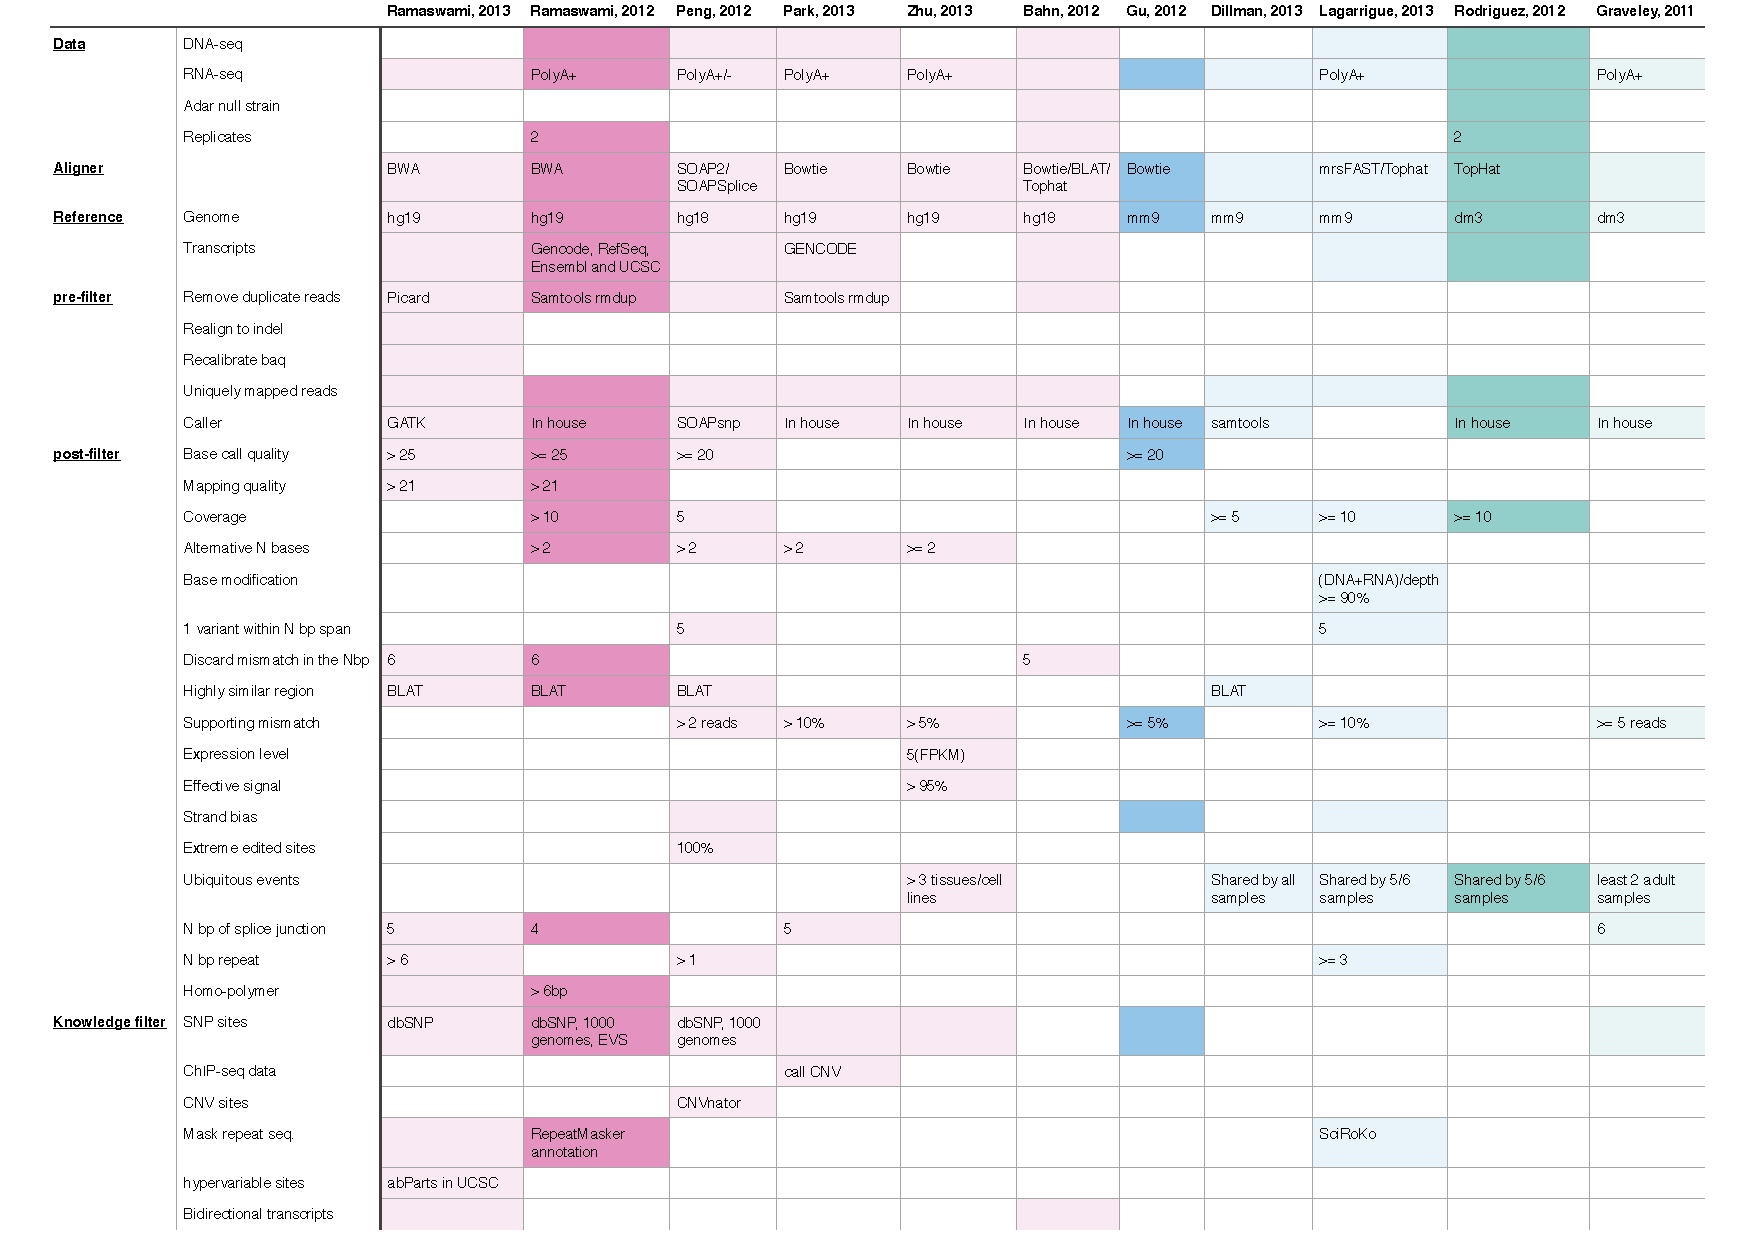
\includegraphics[width=1.1 \hsize]{methods_table.pdf}
	\end{center}
	\vspace*{-1cm}
	\caption{精度検証に用いた手法の詳細}
\end{figure}

\newpage

\section{議論}
先行研究においては、T-to-GやC-to-Aなど全塩基置換の個数を集計し、全体の分布においてA-to-Gへの置換が濃縮されたピークとして見られること、またはmodENCODEやDARNEDのデータを使い、既知の報告例との一致の割合を示すことにより、検出手法の妥当性を示してきた。検出手法ごとに異なったデータや方法で検出精度の妥当性を評価しており、検出手法を比較することは困難であった。このような問題に対し、本研究は、情報検索の分野で用いられてきた適合率・再現率およびF値と呼ばれる精度評価の指標を導入し、RNA editingサイトの検出手法の精
度を定量化し、異なる複数の手法の比較を可能にした。
\par
ヒトにおいては、リードのマッピングにおいては参照配列をゲノムに限らず、複数の遺伝子モデルを用いたマッピングが高精度化に寄与する可能性が示唆された。
\par
マウスにおける検出手法の精度評価の議論。
\par
ショウジョウバエにおける検出手法の議論。
\par
高精度な検出に寄与すると考えられた実験デザインについての議論。
\par
適合率および再現率によって、異なる検出手法を比較することには成功した。しかし、より正確な性能評価には、全ての手法において同一のRNA-seqデータを使って再解析する必要があると考えている。本解析では、入力となるRNA-seqデータと手法の双方が先行研究ごとに異なり、純粋に手法のみの比較が行えていない可能性が考えられる。解析対象となったRNA-seqデータと検出手法の影響を明確に分離し、RNA-seqデータを比較する全ての手法で同一にした上で、性能評価を行う必要があるだろう。そのためには、ENCODEプロジェクトなどの豊富なデータを用いて、純粋な手法の比較を行うことが望まれる。

